%%%%%%%%%%%%%%%%%%%%%%%%%%%%%%%%%%%%%%%%%
% University/School Laboratory Report
% LaTeX Template
% Version 3.1 (25/3/14)
%
% This template has been downloaded from:
% http://www.LaTeXTemplates.com
%
% Original author:
% Linux and Unix Users Group at Virginia Tech Wiki 
% (https://vtluug.org/wiki/Example_LaTeX_chem_lab_report)
%
% License:
% CC BY-NC-SA 3.0 (http://creativecommons.org/licenses/by-nc-sa/3.0/)
%
%%%%%%%%%%%%%%%%%%%%%%%%%%%%%%%%%%%%%%%%%

%----------------------------------------------------------------------------------------
%	PACKAGES AND DOCUMENT CONFIGURATIONS
%----------------------------------------------------------------------------------------

\documentclass{article}

\usepackage[version=3]{mhchem} % Package for chemical equation typesetting
\usepackage{siunitx} % Provides the \SI{}{} and \si{} command for typesetting SI units
\usepackage{graphicx} % Required for the inclusion of images
\usepackage{natbib} % Required to change bibliography style to APA
\usepackage{amsmath} % Required for some math elements 
\usepackage{enumerate}
\usepackage[utf8x]{inputenc}
\usepackage{hyperref}


\setlength\parindent{0pt} % Removes all indentation from paragraphs

\renewcommand{\labelenumi}{\alph{enumi}.} % Make numbering in the enumerate environment by letter rather than number (e.g. section 6)

%\usepackage{times} % Uncomment to use the Times New Roman font

%----------------------------------------------------------------------------------------
%	DOCUMENT INFORMATION
%----------------------------------------------------------------------------------------

\title{Relazione esercitazione di laboratorio - Parte 1
\\ MeMOC
\\ Anno 2014/2015}

\date{} % Date for the report
\author{} % Author name

\begin{document}

\maketitle % Insert the title, author and date

\begin{center}
\begin{tabular}{l r}
Autore & Marco Baesso \\ % Date the experiment was performed
Matricola: & 1082306 \\ % Partner names
%& Mary Smith \\
%Instructor: & Professor Smith % Instructor/supervisor
\end{tabular}
\end{center}

% If you wish to include an abstract, uncomment the lines below
% \begin{abstract}
% Abstract text
% \end{abstract}

%----------------------------------------------------------------------------------------
%	SECTION 1
%----------------------------------------------------------------------------------------

\section{Scelte implementative}
In questa sezione vengono riportate informazioni relative alla implementazione del progetto, in particolare relative ai step di compilazione, esecuzione e alla parte di codifica.

\subsection{Linguaggio usato}
\label{linguaggio}
L'esercitazione è stata implementata in \textit{C++} integrando i seguenti framework: \textit{Cplex} e \textit{Qt}. Il primo è stato utilizzato per la risoluzione del problema di minimizzazione proposto; il secondo al fine di agevolare la codifica e la gestione dei dati del problema.

\subsection{Compilazione}
\label{compilazione}
Per la compilazione del progetto eseguire i seguenti passi:
\begin{enumerate}[I]
\item aprire il terminale;
\item posizionarsi nella cartella contenente l'esercitazione (cartella \textit{root} d'ora in poi);
\item eseguire il seguente comando: sh compila.sh.
\end{enumerate}

L'eseguibile, quindi, apparirà nella \textit{root} riportando il nome \textit{tsp\_pannelli\_forati}.

\subsection{Input e Output}
\label{input e output}
\subsubsection{Input}
L'input del problema deve essere un file che contiene dei nodi espressi come coordinate nel piano cartesiano. \\
\textbf{La grammatica per i dati di input è quindi una serie di punti x,y separati dal carattere di a capo.} \\
Il file tsp\_pannelli\_forati può essere eseguito in 2 modi:
\begin{enumerate}[I]
\item \textit{./tsp\_pannelli\_forati default}\\
Quindi passando come primo argomento la stringa default il programma andrà a prendere il file \textit{default} che troverà in \textit{data/}.\\
Questo è il modo standard ovvero, basterà prendere un tsp che rispetti la grammatica di input e il programma risolverà il tsp.
\item \textit{./tsp\_pannelli\_forati [classe\_tsp][numero\_nodi][dispersione\_nodi]}, dove i parametri hanno la seguente funzione:
\begin{itemize}
\item \textbf{[classe\_tsp]}: può assumere valore \textit{cerchio} o \textit{randoms}; quindi nel primo caso il tsp genera dei dati che prestano alla forma di una circonferenza; nel secondo caso i dati saranno dei punti casuali nel piano;
\item \textbf{[numero\_nodi]}: indica il numero di nodi che devono essere dati al risolutore in input;
\item \textbf{[dispersione\_nodi]}: questo parametro indica la dimensione dell'asse delle ascisse su cui scegliere \textit{numero\_nodi} nodi per la classe \textit{cerchio}; analogamente per la classe \textit{randoms}. 
\end{itemize}
\end{enumerate}

\subsubsection{Output}
Quando il tsp è stato risolto nella \textit{root} apparirà il file \textit{output.txt} che contiene i valori delle variabili del tsp \textbf{non nulle}; il tempo impiegato per eseguire e il valore della funzione obiettivo.

\subsection{Struttura del codice}
Nel file \textit{main.cpp} viene riportata la procedura \textit{main} le cui principali procedure richiamate sono:
\begin{description}
\item \textbf{genera\_nodi\_problema}; nel caso in cui il programma viene eseguito con modalità non standard vengono generate i nodi del problema in funzione dei parametri di input configurati;
\item \textbf{crea\_variabili}: per la creazione delle variabili sono stati indicizzati gli indici a cui si riferiscono le variabili in una mappa delle dimensioni di num\_nodi*(num\_nodi-1) al fine di non usare le variabili che rappresentano i cappi dato che il cappio non è utile al problema.\\
Quindi nell'inidicizzazione per riferirsi al nodo i,j occorre porre attenzione al fatto che se j$>$i nella mappa l'indice che contiene la posizione in cui CPLEX ha memorizzato il nodo i\_j è in i\_j-1;    
\item \textbf{crea\_vincoli}: utilizzata per la creazione dei vincoli del problema.
\end{description}  

\section{Test}
In questa sezione vengono riportati i risultati ottenuti eseguendo il risolutore prima su delle classi specifiche, poi su dataset specifici reperibili online al seguente indirizzo: \url{http://www.math.uwaterloo.ca/tsp/vlsi/index.html#XQF131}


\subsection{Classe cerchio}
\begin{table}[h]
\centering
\begin{tabular}{c | c | c}
\hline \hline
\textbf{Numero nodi} & \textbf{Dispersione} & \textbf{Tempo (secondi)} \\
\hline
25 & 25 & 3 \\
\hline
25 & 100 & 3 \\ \\
\hline
\hline
35 & 35 & 4 \\
\hline
35 & 100 & 5 \\ \\
\hline
\hline
40 & 40 & 7 \\
\hline
40 & 150 & 18 \\ \\
\hline
\hline
45 & 150 & 37 \\
\hline
45 & 180 & 34 \\
\hline
45 & 250 & 19 \\ \\
\hline
\hline
50 & 50 & 85 \\
\hline
50 & 180 & 44 \\ \\
\hline
\hline
55 & 55 & 83  \\ \\
\hline
\hline
60 & 70 & 809  \\
\hline
60 & 100 & 738   \\ \\
\hline
70 & 70 & 821   \\ \\
\hline
\hline
90 & 90 & \textbf{N.D.} \\
\hline
\end{tabular}
\end{table}

\newpage
\subsection{Classe randoms}
\begin{table}[h]
\centering
\begin{tabular}{c | c | c}
\hline \hline
\textbf{Numero nodi} & \textbf{Dispersione} & \textbf{Tempo (secondi)} \\
\hline
20 & 20 & 1 \\ \\
\hline
\hline
35 & 35 & 17 \\
\hline
35 & 150 & 20 \\ \\
\hline
\hline
40 & 40 & 28 \\
\hline
40 & 100 & 27 \\
\hline
40 & 1000 & 58 \\ \\
\hline
\hline
45 & 45 & 52 \\
\hline
45 & 300 & 45 \\ \\
\hline
\hline
60 & 60 & 220 \\
\hline
60 & 400 & 169 \\ \\
\hline
\hline
80 & 80 & 286 \\ \\
\hline
\hline
95 & 105 & \textbf{N.D.} \\
\hline
\end{tabular}
\end{table}

Per le classi cerchio e randoms si può notare che a parità numero di nodi la dispersione influenza il tempo di esecuzione; se si prende per esempio il test case per 45 nodi per la classe cerchio si può notare che il tempo di esecuzione decresce; questo è probabilmente dovuto al fatto che aumentando la dispersione i punti scelti tendono ad allontanarsi da quello che sarebbe il comportamento tipico rispetto alla loro classe di appartenenza.
\\
Considerando i dati sopra riportati si può notare che se il numero di nodi è \textit{circa 50} il risolutore riesce a risolvere il tsp in un tempo variabile tra \textit{\textbf{1 e 3 minuti}}.
Mentre per un numero di nodi maggiore il comportamento è variabile a seconda della classe di appartenenza; per esempio per un numero di nodi tra \textit{60 e 70} il tempo di esecuzione per la classe cerchio è superiore ai \textit{\textbf{10 minuti}}. Mentre per la classe randoms fino ad 80 nodi il tempo di esecuzione è inferiore ai \textit{\textbf{5 minuti}}. \\
Per numero di nodi maggiore di 80 per entrambe le classi non è stato calcolato il tempo di esecuzione anche se guardando ai dati ottenuti si può notare che per la classe cerchio il tempo di esecuzione con una buona probabilità sarà maggiore rispetto al tempo che verrà impiegato per un tsp appartenente alla classe randoms. 


\newpage

\subsection{DataSet per TSP}
\label{sec:datasetTSP}
\subsubsection{dataset XQF131}

\begin{figure}[h]
\begin{center}
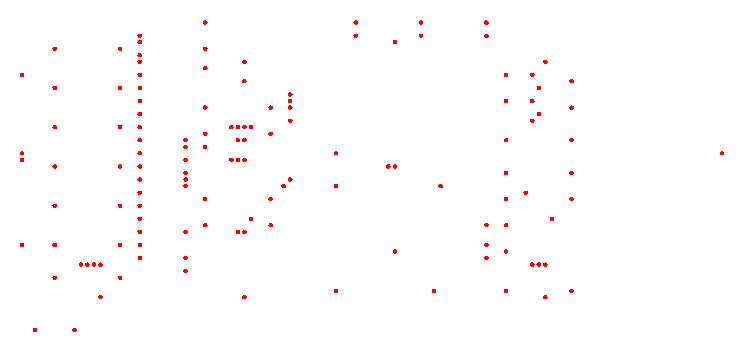
\includegraphics[scale=0.5]{img/xqf131.png} % Include the image placeholder.png
\caption{dataset xqf131}
\end{center}
\end{figure}

\begin{table}[h]
\centering
\begin{tabular}{c | c}
\hline \hline
\textbf{Numero nodi} & \textbf{Tempo (secondi)} \\
\hline
35 & 3 \\
\hline
45 & 10 \\
\hline
55 & 50 \\
\hline
70 & 144 \\
\hline
100 & \textbf{N.D} \\
\hline

\end{tabular}
\end{table}

\newpage
\subsubsection{dataset PMA343}

\begin{figure}[h]
\begin{center}
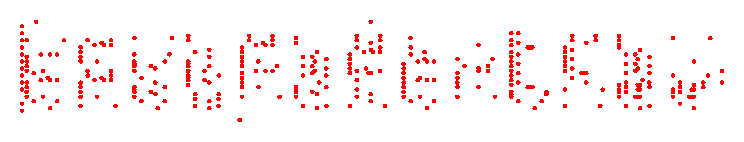
\includegraphics[scale=0.5]{img/pma343.png} % Include the image placeholder.png
\caption{dataset pma343}
\end{center}
\end{figure}

\begin{table}[h]
\centering
\begin{tabular}{c | c}
\hline \hline
\textbf{Numero nodi} & \textbf{Tempo (secondi)} \\
\hline
50 & 16 \\
\hline
75 & 165 \\
\hline
100 & 1021 \\
\hline
120 & \textbf{N.D.} \\
\hline
\end{tabular}
\end{table}

\newpage
\subsubsection{dataset PBL395}

\begin{figure}[h!]
\begin{center}
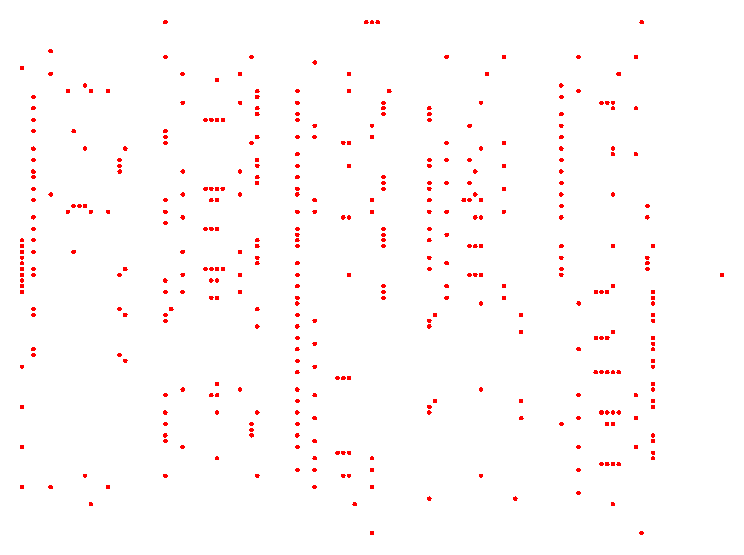
\includegraphics[scale=0.5]{img/pbl395.png} % Include the image placeholder.png
\caption{dataset pbl395}
\end{center}
\end{figure}

\begin{table}[h]
\centering
\begin{tabular}{c | c}
\hline \hline
\textbf{Numero nodi} & \textbf{Tempo (secondi)} \\
\hline
40 & 88 \\
\hline
55 & 94 \\
\hline
70 & 176 \\
\hline
85 & \textbf{N.D.} \\
\hline
\end{tabular}
\end{table}

Per i tsp della sezione~\nameref{sec:datasetTSP} è stato riportato il plot dei punti dell'intero dataset; mentre i test sono stati eseguiti su un numero limitato di nodi prendendo per ogni tsp i primi \textit{k} nodi presi in ordine di ascissa crescente.\\
Dal plot dei punti si può notare l'affinità con le schede perforate, quindi di utilità per i casi pratici e in particolare per l'applicazione nel dominio del problema richiesto nell'esercitazione.\\
Dai dataset presi si può notare che fino circa a 100 nodi il tempo di esecuzione è inferiore ai \textbf{\textit{17 minuti}}.

%----------------------------------------------------------------------------------------
%	BIBLIOGRAPHY
%----------------------------------------------------------------------------------------

%\bibliographystyle{apalike}

%\bibliography{sample}

%----------------------------------------------------------------------------------------


\end{document}